\documentclass{article}
\usepackage{../../Self_Style}

\title{Phys 20BL Week7/8 Out of Lab: RCL Circuits}
\author{Zih-Yu Hsieh}
\date{\today}

\begin{document}
\maketitle

\tableofcontents

\newpage

\section{Physical Model for RC Circuit}
\subsection{Lab Guide Model}
Let's start with what the lab guide says:

Given that the voltage of a capacitor is linearly proportional to the charge obtained on the capacaitor, if the proportionality constant is denoted as ``capacitance'' $C$, then it provides the following equation, with $Q$ being the charge (unit: Coulomb C) and $V$ being the voltage (unit: Volt V):
\begin{align}
    Q=CV
\end{align}
Also, by definition the rate of change of charge $Q$ with respect to the time is the current of the system $I$ (unit: Ampere A). Which, with capacitance $C$ remaining constant, the above equation implies the following:
\begin{align}
    I(t)=\frac{dQ}{dt} = C\frac{dV}{dt}
\end{align}
Finally, using Ohm's Law, with $I=V/R$, where $R$ is the resistance (unit: Ohms $\Omega$). If the circuit has fixed resistance $R$, then one derives the following equation:
\begin{align}
    V(t)=I(t)R = RC \frac{dV}{dt}
\end{align}

\textbf{Remark:} This only considers the information across the capacitor, and fails to consider the general setup. Which, it can never solve the desired model on its own (as for $R,C>0$ as assumption, this differential equation provides $V(t)=V_0e^{t/(R C)}$, which is exponentially growing, failed to capture the general situation). So, let's include some more information.

\hfil

\subsection{Derivation for RC Circuits}
Here, we'll fix a constant voltage source $V_s>0$, $V(t)$ represents the voltage across the capacitor, $I(t)$ represents the total current in the circuit, $C$ represents the constant capacitance of the capacitor, and $R$ represents the constant resistance. 

In an RC Circuit, since the voltage across the resistance and across the capacitance should sum up to the provided voltage $V_0$, hence one has voltage across the resistance being $V_0-V(t)$. Also, by Ohm's Law, the voltage across the resistance is $R I(t)$, hence one has the equation $V_0-V(t)=R I(t)$, or $R I(t)+V(t)=V_0$.

Finally, notice that $I(t)=\frac{dQ}{dt}$, where $Q(t)$ is the charge of the capacitor. Which, if $C,V(t)$ are the capacitance and voltage across the capacitor respectively, then $Q(t)=C V(t)$, hence $I(t)=\frac{dQ}{dt} = C \frac{dV}{dt}$.

Combine the two parts, we get the following differential equation:
\begin{align}
    RC\frac{dV}{dt}+V(t)=V_s
\end{align}
As a side note, for the case $V_s<0$, this differential equation still works (just in general it's convenient to choose the direction where $V_s>0$).

\hfil

As of example, there are two functions (\textbf{Equation 1 \& 2} in the In Lab portion) to consider:
\begin{align}
    &V(t)=V_0 (1-e^{-t/\tau_\text{step}})\\
    &V(t)=V_0^{-t/\tau_\text{nat}}
\end{align}
Let's try and solve these in terms of differential equations with initial conditions.

\newpage

\subsubsection{Solution for Equation 1}

Given the equation $V(t)=V_0(1-e^{-t/\tau_\text{step}})$, it models the circuit with the following condition:
\begin{itemize}
    \item A fixed positive voltage source $V_s=V_0>0$.
    \item The capacitor is initially with no charge, namely $Q(0) = C\cdot V(0)=0$. Then, it implies $V(0)=0$.
    \item The resistance $R>0$ and capacitance $C>0$ of the circuit are fixed.
\end{itemize}
Which, solving the above differential equation under this condition, we get:
\begin{align}
    &RC\frac{dV}{dt}+V(t)=V_0\\
    &\implies \frac{dV}{dt}+\frac{1}{RC}V(t)=\frac{V_0}{RC}\\
    &\implies \frac{dV}{dt}e^{t/(RC)}+V(t)\cdot \frac{1}{RC}e^{t/(RC)} = \frac{V_0}{RC}e^{t/(RC)}\\
    &\implies \frac{d}{dt}\left(V(t)\cdot e^{t/(RC)}\right)=\frac{V_0}{RC}e^{t/(RC)}\\
    &\implies V(t)\cdot e^{t/(RC)} = V_0e^{t/(RC)} + D\\
    &\implies V(t) = V_0+De^{-t/(RC)}
\end{align}
Under the initial condition $V(0)=0$, one has $V_0+D=0$, or $D=-V_0$. Hence, the solution is given as follow:
\begin{align}
    V(t)=V_0\left(1-e^{-t/(RC)}\right)
\end{align}
So, one has the step response time constant $\tau_\text{step} = RC$.

\hfil

\subsubsection{Solution for Equation 2}

Given the equation $V(t)=V_0e^{-t/\tau_\text{nat}}$. Notice that it's under the following condition:
\begin{itemize}
    \item Zero voltage source $V_s=0$ (modeling the situation where voltage source is turned off).
    \item The capacitor is fully charged initially, say $V(0)=V_0$ (normally meaning the voltage source before getting turned off).
\end{itemize}
Which, solving th above differential equation under this condition, we get:
\begin{align}
    &RC\frac{dV}{dt}+V(t)=0\\
    &\implies \frac{dV}{dt}=-\frac{1}{RC}V(t)\\
    &\implies V(t)=De^{-t/(RC)}
\end{align}
Under the initial condition $V(t)=V_0$, oe has $D=V_0$. Hence, the solution is given as follow:
\begin{align}
    V(t)=V_0e^{-t/(RC)}
\end{align}
So, one has the natural response time constant $\tau_\text{nat}=RC$ again.

\newpage

\section{Physical Model for LRC Circuit}

This section is more related to the modification of experiments I've done.

Let's recall that for an inductor with fixed inductance $L$, when a current passes through it (assuming the current is a differentiable function), one has the following voltage change across the inductance:
\begin{align}
    V = -L\frac{dI}{dt}
\end{align}
Where, the voltage change is the voltage after the current passes through the inductor, subtracted by the voltage before the current passes through the inductor. In particular, its positive version $L\frac{dI}{dt}$ can be viewed as the voltage difference across the circuit.

\hfil

\subsection{Series and Parallel for Inductance}

Suppose there are $n$ inductors involved, with inductance $L_1,...,L_n$ respectively. There are two cases to consider:
\begin{itemize}
    \item If the inductors are in series, then notice they share a common current $I(t)$ (assume differentiability). Hence, across the $i$th inductor the voltage change is $V_i = -L_i\frac{dI}{dt}$, and the voltage change across the whole series arrangement is $V = \sum_{i=1}^nV_i = -\left(\sum_{i=1}^nL_i\right)\frac{dI}{dt}$. 
    
    Which, if view the whole series arrangement with a total inductance $L$, then one has $V = -L\frac{dI}{dt}$, hence in general $L = \sum_{i=1}^n L_i$.
    \begin{figure}[h!]
        \centering
        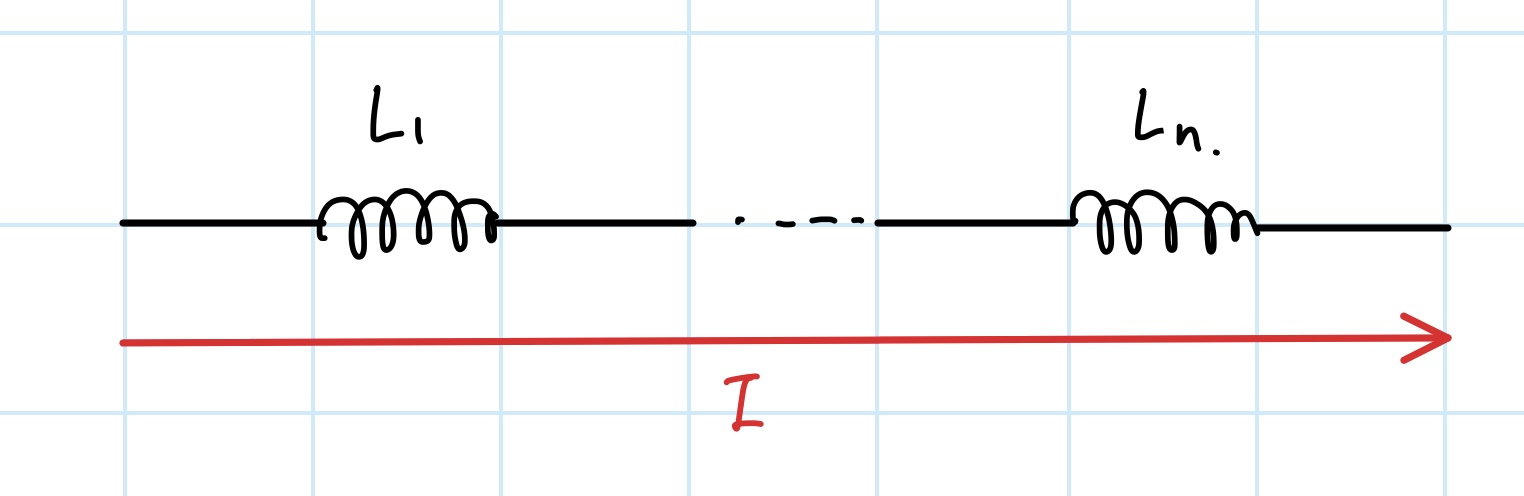
\includegraphics[width=120mm]{series.jpg}
        \caption{Inductors in Series}
    \end{figure}

    \hfil

    \item If the inductors are in parallel, let $I_i$ be the current passing through the $i$th inductor, then one has the total current $I=\sum_{i=1}^{n}I_i$. Then, notice they all share the same voltage change, say $V$. Hence, across the $i$th inductor one has voltage change $V=-L_i\frac{dI_i}{dt}$, or $-\frac{dI_i}{dt}=\frac{V}{L_i}$.
    
    As a result, the total current satisfies $-\frac{dI}{dt}=-\sum_{i=1}^n\frac{dI_i}{dt} = \sum_{i=1}^n\frac{V}{L_i}$, hence if $L$ is a total inductance of the parallel arrangement, one has $V = -L\frac{dI}{dt} = V\cdot L\sum_{i=1}^{n}\frac{1}{L_i}$. In the general (nontrivial) situation, one has $\frac{1}{L}=\sum_{i=1}^n\frac{1}{L_i}$.
    \begin{figure}[h!]
        \centering
        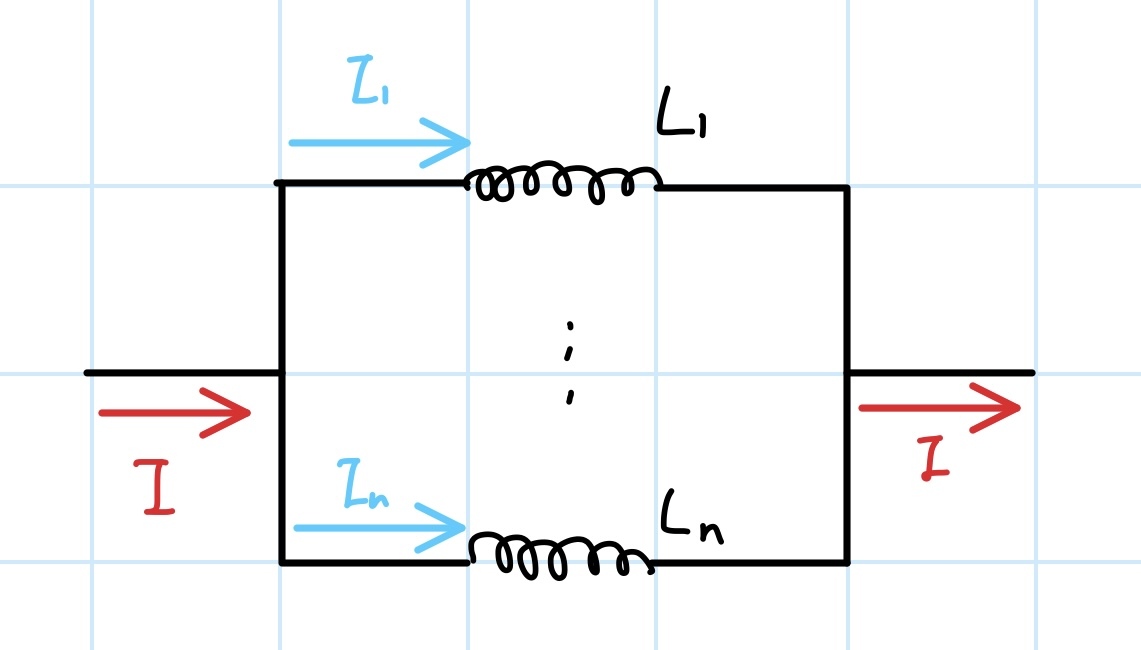
\includegraphics[width=100mm]{parallel.jpg}
        \caption{Inductors in Parallel}
    \end{figure}
\end{itemize}

\newpage

Hence, we concluded that under ideal situation, the current E\&M Models predicted the total inductance to be:
\begin{itemize}
    \item $L=\sum L_i$, given that the inductors are in series.
    \item $\frac{1}{L}=\sum \frac{1}{L_i}$, given that the inductors are in parallel.
\end{itemize}

\hfil

\subsection{Differential Equation for LRC Circuit}

Now, let $V_s>0$ represents a (fixed) voltage source, $V(t)$ be the voltage across the capacitance, $L,R,C$ represents the inductance, resistance, and capacitance of the LRC circuit respectively. Then, with $I(t)=\frac{dQ}{dt}=C\frac{dV}{dt}$ be the current, one has $\frac{dI}{dt} = C\frac{d^2V}{dt^2}$.

Given the voltage across the inductor $L\frac{dI}{dt} = LC \frac{d^2V}{dt^2}$, the voltage across the resistance $RI(t)=RC\frac{dV}{dt}$, and the voltage across the capacitance $V(t)$, since they need to sum up to the fixed voltage source $V_s$, one arrives at the following differential equation:
\begin{align}
    LC\frac{d^2V}{dt^2}+RC\frac{dV}{dt}+V(t)=V_s\ \implies\ \frac{d^2V}{dt^2}+\frac{R}{L}\frac{dV}{dt}+\frac{1}{LC}V(t)=\frac{V_s}{LC}
\end{align}
Which, given the characteristic equation $r^2+\frac{R}{L}r+\frac{1}{LC}=0$, the roots are given by $r = -\frac{R}{2L}\pm \sqrt{\left(\frac{R}{2L}\right)^2-\frac{1}{LC}}$ (which can be complex or real, dependent on the given value $L$). Which, labeling $w := \sqrt{\left(\frac{R}{2L}\right)^2-\frac{1}{LC}}$, the general solution to the homogeneous equation is:
\begin{align}
    V_h(t) = e^{-Rt/(2L)}\left(Ae^{w t}+Be^{-wt}\right)
\end{align}
Now, with the inhomogeneous part being constant $\frac{V_s}{LC}$, $V_p(t)=\frac{V_s}{LC}$ is a particular solution satisfying this differential equation, then the full solution is given as follow:
\begin{align}
    V(t)=V_s + e^{-Rt/(2L)}\left(Ae^{w t}+Be^{-wt}\right)
\end{align}
Finally, to obtain the voltage across the inductor, it's given as $LC \frac{d^2V}{dt^2}$, which can be solved once given all the coefficients.

\hfil

\subsection{Model for this Experiment}

In our experiment, the provided voltage source is a square wave. However, realistically to observe the behavior of the LRC circuit, one only needs to observe the voltage within half a cycle, so one can treat the voltage source as $0$ for $t<0$, and $V_s=V_0$ for $t\geq 0$.

For simplicity of model, we'll also assume that within a short amount of time right after the voltage source is switched, the capacitance is not charged (which, it's approximated by $V(0)=0$, or initially there's no voltage change across capacitance); on the other hand, one will also assume the voltage difference is given solely by the resistance, so $V_0 = R I(0) = R C \frac{dV}{dt}\bigg|_{t=0}$. Hence, $\frac{dV}{dt}\bigg|_{t=0} = \frac{V_0}{RC}$.

\hfil

As for solution, notice that plugin to the general solution, one has the fllowing:
\begin{align}
    0=V(0)=V_0 + A+B\ \implies\ A+B = -V_0
\end{align}
\begin{align}
    \frac{V_0}{RC}=\frac{dV}{dt}\bigg|_{t=0} = -\frac{R}{2L}(A+B)+w(A-B)\ \implies\ A-B = \frac{1}{w}\left(\frac{1}{RC}-\frac{R}{2L}\right)V_0
\end{align}
(Note: Here we assume $w\neq 0$, as for basically $100\%$ of the $L,R,C$ combinations, $w\neq 0$).

Hence, one obtains the following two coefficients:
\begin{align}
    A = \frac{1}{2w}\left(\frac{1}{RC}-\frac{R}{2L}-w\right)V_0,\quad B = -\frac{1}{2w}\left(\frac{1}{RC}-\frac{R}{2L}+w\right)V_0
\end{align}
Which, if $w$ is imaginary, the solution for $V$ will be taken as the real portion.

\newpage

\section{Week 7 Portion - RC Circuit}


\end{document}